\section{Programa BPMN transformacijai į užduočių diagramą}


Vienas iš šio darbo tikslų yra programa, demonstruojanti algoritmo \BPMN{} transformacijai į užduočių diagramą, veikimą. Programos įeigai pasirinktas \BPMN{} išplėtimas \DVCM{} modelis, išeiga – užduočių diagrama. Algoritmas aprašytas \ref{section:main_use_cases_from_bpmn} skyriuje. Programos realizacija yra „github“ sistemoje. Ten galima rasti:
\begin{enumerate}
  \item Programos kodą \href{https://github.com/Aleksandras-Sivkovas/diagrams-editor-app}{https://github.com/Aleksandras-Sivkovas/diagrams-editor-app}.
  \item Sutransliuotą demo versiją \href{https://aleksandras-sivkovas.github.io/diagrams-editor-app/}{https://aleksandras-sivkovas.github.io/diagrams-editor-app/}.
  \item Pavyzdinį \JSON{} formato duomenų failą, kurį galima importuoti programoje arba generuoti iš jo užduočių diagramas \href{https://aleksandras-sivkovas.github.io/diagrams-editor-app/dvcm.json}{https://aleksandras-sivkovas.github.io/diagrams-editor-app/dvcm.json}.
\end{enumerate}
Algoritmo aprašyto \ref{section:main_use_cases_from_bpmn} skyriuje realizaciją „Javascript“ kalba pateikiama \ref{appendix:pseudocode_implementation} priede.

\subsection{Funkciniai reikalavimai programai}

Čia aprašomi demonstracinės programos funkciniai reikalavimai. Jie pateikiami užduočių diagramos pavidalu (\ref{img:program_functional_requirements} pav.) bei aprašomi \ref{tab:program_re_dvcm_creation}, \ref{tab:program_re_dvcm_save} ir \ref{tab:program_re_uc_generation} lentelėse. Šie reikalavimai parodys kokiomis funkcijos galės pasinaudoti naudotojas norėdamas pasižiūrėti algoritmo veikimą.

\begin{figure}[H]
	\centering
	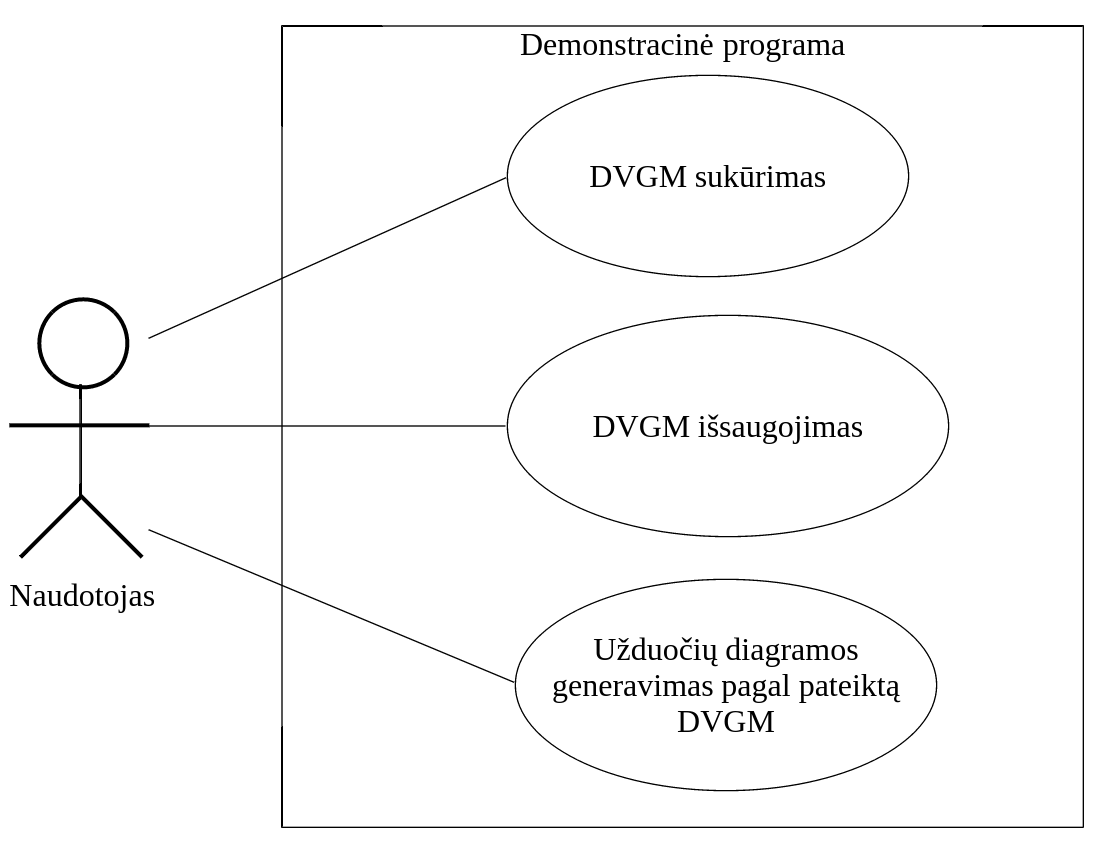
\includegraphics[width=\textwidth]{sections/prototype_app/img/program_functional_requirements}
	\caption{Demonstracinės programos funkciniai reikalavimai.}
	\label{img:program_functional_requirements}
\end{figure}

\begin{center}
    \begin{longtable}{|p{\textwidth}|}
    \caption{\DVCM{} kūrimo naudojimo atvejis}
	\label{tab:program_re_dvcm_creation}
	\\ \hline
    \begin{tabular}{@{}p{3.5cm}p{12cm}}
    	\\
    	\textbf{ID} & NA1
    	\\
    	\textbf{Pavadinimas} & \DVCM{} sukūrimas
    	\\
    \end{tabular}
    \\
    \textbf{Aktoriai}
    \begin{enumerate}
    	\item Naudotojas.
	\end{enumerate}
    \\
    \textbf{Aprašas}

      Naudotojas pasinaudojęs demonstracine programa sukuria \DVCM{}.

    \\
    \textbf{Prieš sąlygos}
    \begin{enumerate}
    	\item Naudotojas yra atidaręs demonstracinės programos langą.
	\end{enumerate}
    \\
    \textbf{Priežastys}
    \begin{enumerate}
    	\item Naudotojas pareikalavo sukurti \DVCM{}.
	\end{enumerate}
    \\
    \textbf{Po sąlygos}
    \begin{enumerate}
    	\item Naudotojas yra sukūręs \DVCM{}.
      \item Naudotojas mato savo sukurtą \DVCM{} demonstracinės programos lange.
	\end{enumerate}
    \\
    \textbf{Pagrindinė užduočių seka}
    \begin{enumerate}
    	\item Demonstracinė programa pateikia interfeisą \DVCM{} kūrimui.
    	\item Naudotojas kuria \DVCM{}.
	\end{enumerate}
    \\
    \textbf{Alternatyvios užduočių sekos}

    \\
    \textbf{Išimtinės užduočių sekos}

    \\
    \\ \hline
    \end{longtable}
\end{center}

\begin{center}
    \begin{longtable}{|p{\textwidth}|}
    \caption{\DVCM{} saugojimo naudojimo atvejis}
	\label{tab:program_re_dvcm_save}
	\\ \hline
    \begin{tabular}{@{}p{3.5cm}p{12cm}}
    	\\
    	\textbf{ID} & NA2
    	\\
    	\textbf{Pavadinimas} & \DVCM{} išsaugojimas
    	\\
    \end{tabular}
    \\
    \textbf{Aktoriai}
    \begin{enumerate}
    	\item Naudotojas.
	\end{enumerate}
    \\
    \textbf{Aprašas}

      Naudotojas išsaugo demonstracine programa sukurtą \DVCM{}.

    \\
    \textbf{Prieš sąlygos}
    \begin{enumerate}
    	\item Naudotojas yra atidaręs \DVCM{} kūrimo interfeisą.
	\end{enumerate}
    \\
    \textbf{Priežastys}
    \begin{enumerate}
    	\item Naudotojas pareikalavo išsaugoti \DVCM{}.
	\end{enumerate}
    \\
    \textbf{Po sąlygos}
    \begin{enumerate}
    	\item Naudotojas yra išsaugojęs \DVCM{}.
      \item Naudotojas žino, kad \DVCM{} išsaugotas.
	\end{enumerate}
    \\
    \textbf{Pagrindinė užduočių seka}
    \begin{enumerate}
    	\item Demonstracinė programa pateikia išsaugojimo formatus.
    	\item Naudotojas pasirenka kaip saugoti \DVCM{}.
			\item Demonstracinė programa pareikalauja išsaugojimo informacijos.
			\item Naudotojas įveda išsaugojimo informaciją.
      \item Demonstracinė programa išsaugo \DVCM{}.
      \item Demonstracinė programa patvirtina, kad \DVCM{} išsaugotas.
	\end{enumerate}
    \\
    \textbf{Alternatyvios užduočių sekos}

    \\
    \textbf{Išimtinės užduočių sekos}
			\newlist{seka}{enumerate}{3}
			\setlist[seka]{label*=\arabic*.,leftmargin=2em}
			\setlist[seka,1]{label=*.\arabic*.,leftmargin=2em}
			\begin{seka}
					\item Naudotojas atsisako išsaugoti \DVCM{}.
					\begin{seka}
						\item Naudotojas pateikia išsaugoti atsisakymą.
						\item Demonstracinė programa nebereikalauja duomenų.
					\end{seka}
			\end{seka}
    \\
    \\ \hline
    \end{longtable}
\end{center}

\begin{center}
    \begin{longtable}{|p{\textwidth}|}
    \caption{Užduočių diagramos generavimo pagal pateiktą \DVCM{} modelį naudojimo atvejis}
	\label{tab:program_re_uc_generation}
	\\ \hline
    \begin{tabular}{@{}p{3.5cm}p{12cm}}
    	\\
    	\textbf{ID} & NA3
    	\\
    	\textbf{Pavadinimas} & Užduočių diagramos generavimas pagal pateiktą \DVCM{}
    	\\
    \end{tabular}
    \\
    \textbf{Aktoriai}
    \begin{enumerate}
    	\item Naudotojas.
	\end{enumerate}
    \\
    \textbf{Aprašas}

      Naudotojas demonstracinei programai programa pateikia \DVCM{} ir programa sugeneruoja užduočių diagramą.

    \\
    \textbf{Prieš sąlygos}
    \begin{enumerate}
    	\item Naudotojas yra atidaręs programos langą.
	\end{enumerate}
    \\
    \textbf{Priežastys}
    \begin{enumerate}
    	\item Naudotojas pareikalavo sugeneruoti užduočių diagramą iš \DVCM{}.
	\end{enumerate}
    \\
    \textbf{Po sąlygos}
    \begin{enumerate}
    	\item Demonstracinėje programoje yra užduočių diagramos duomenys.
      \item Naudotojas mato sugeneruotą užduočių diagramą Demonstracinės programos lange.
	\end{enumerate}
    \\
    \textbf{Pagrindinė užduočių seka}
    \begin{enumerate}
      \item Demonstracinė programa pateikia užduočių diagramos generavimo iš \DVCM{} variantus.
      \item Naudotojas pasirenka generuoti bendrą diagramą iš \DVCM{}. \label{seka:re_generate_choose_way}
    	\item Demonstracinė programa pateikia interfeisą \DVCM{} įvedimui.
    	\item Naudotojas įveda \DVCM{}.
      \item Demonstracinė programa sugeneruoja užduočių diagramos modelį.
      \item Demonstracinė programa pavaizduoja užduočių diagramą lange.
	\end{enumerate}
    \\
    \textbf{Alternatyvios užduočių sekos}
			\newlist{seka}{enumerate}{3}
			\setlist[seka]{label*=\arabic*.,leftmargin=2em}
			\setlist[seka,1]{label=\ref{seka:re_generate_choose_way}.\arabic*.,leftmargin=2em}
			\begin{seka}
					\item Naudotojas Naudotojas pasirenka iš \DVCM{} sugeneruotą diagramą rodyti po vieną transakciją.
			\end{seka}
    \\
    \textbf{Išimtinės užduočių sekos}
			\newlist{seka}{enumerate}{3}
			\setlist[seka]{label*=\arabic*.,leftmargin=2em}
			\setlist[seka,1]{label=*.\arabic*.,leftmargin=2em}
			\begin{seka}
					\item Naudotojas atsisako generavimo.
					\begin{seka}
						\item Naudotojas pateikia generavimo atsisakymą.
						\item Demonstracinė programa nebereikalauja duomenų.
					\end{seka}
			\end{seka}
    \\
    \\ \hline
    \end{longtable}
\end{center}

\subsection{Technologijos pasirinktos programos įgyvendinimui}

\subsubsection{Javascript}

Programai įgyvendinti pasirinkta „Javascript“ programavimo kalba. Kadangi reikės atvaizduoti diagramas buvo nuspręsta atlikti tai panaudojant HTML galimybes.  „Javascript“ yra aukšto lygio programavimo kalba. Naujausios jos versijos yra objektiškai orientuotos ir pateikia nemažai kitų aukšto lygio abstrakcijų. Ši kalba yra silpnai tipizuota, objektų išplėtimams naudoja prototipus. „Javascript“ suteikia naršyklių rodomiems puslapiams dinamiškumą. Ilgą laiką ji buvo naudojama tik tam, bet kalbai išpopuliarėjus, ją imta taikyti ir srityse kaip serverinės ar net darbastalio programos. „Javascript“ naudojama kaip interpretuojama programavimo kalba. Interpretavimo standartas „ECMAScript“ buvo išleistas 1997 metais, nuo to laiko jis smarkiai pasikeitė. 2018 metais labiausiai naršyklių pilnai palaikomas yra 5 standartas, šiame darbe rašomas kodas bus transliuojamas į jį.
%Programa yra pilnai klientinės puses (client side), ji neturi serverinės dalies (backend), yra galimybė generuoti failus sukurtiems duomenims saugoti. Failai yra JSON arba JPG formato.

Programos „Javascript“ kodui rašyti pasirinkta 6 „ECMAScript“ versija \cite{EcmaScript}.

\subsubsection{Node.js}

Pasirinkta atviro kodo „Node.js“ programavimo aplinka \cite{nodeJs}. Ši aplinka pritaikyta dirbti su „Javascript“ projektais. Išoriniams paketams tvarkyti pasirinkta atviro kodo „NPM“ paketų tvarkyklė \cite{npmWebsite}. Ši tvarkyklė padeda tvarkyti „Javascript“ paketų versijas. Ji buvo pasirinkta nes yra pagrindinė „Node.js“ aplinkos paketų tvarkyklė.


\subsubsection{Webpack}

Programos modelių surinkimas ir transliavimas aprašomas naudojant atviro kodo „Javascript“ modulių surinkimo bibliotekos „Webpack“ konfiguraciją \cite{webpack}. Ji leidžia pasirinkti kokie moduliai ir kokiu būdu turi būti surinkti ir transliuoti. „Webpack“ naudojamas surinkti „Javascript“ projektą iš daugybės modulių ir transliuoti juos taip, kad palaikytų norimą versiją. Šiuo atveju „Javascript“ 6 standarto kodas transliavimas į 5, kad veiktų naršyklėse.

\subsubsection{Babel}

Programos kodas transliuojamas atviro kodo transliatoriumi „Babel“, kuris naudojamas kaip „Webpack“ prijungimas (plugin).


\subsubsection{MobX}

Programa modeliuojama naudojant MVC metodologiją. Modeliui ir kontroleriui pasirinkta atviro kodo „MobX“ modeliavimo biblioteka \cite{githubMobX}. Ji leidžia kurti programos duomenų modelius ir kontroliuoja jų būsenos klausymąsi naudodama „Javascript“ objekto duomenų priskyrimo ir gavimo metodus.

\subsubsection{React}

Programos „MVC“ vaizdavimo dalis kuriama naudojant atviro kodo „React“ biblioteką \cite{reactJs}. Ji pateikia patogų virtualaus dokumento objekto modelio interfeisą kuris pritaikytas veikti vienodai visose naršyklėse ir optimizuoja dokumento objekto modelio atnaujinimus. Taip pat turi patogią sintaksę vaizdo apibrėžimui – „JSX“. „React“ labai gerai integruojasi su „MobX“.

\subsection{Programos veikimo pavyzdžiai}

\lstset{language=Java,keywordstyle={\bfseries \color{blue} \textbf}}

Atidarius programą matomas trumpas jos aprašymas. Programą galima lokalizuoti į konsolę įvedus komandą \inCode{editorModel.locale = "lt_LT"} (priedas \ref{appendix:run_examples_welcome}). Programa pateikia grafinę diagramų atvaizdavimo sąsają, bet jų kūrimui pateikiamas komandinis interfeisas. Komandomis vadinami „window“ objektui priskirti programos objektai (naudojimo pavyzdys: kodas \ref{lst:commands_to_create_dvcm}). Paspaudus mygtuką \uiWord{Naujas} matomas diagramos kūrimo langas (priedas \ref{appendix:run_examples_new}). Pasirinkus \uiWord{\DVCM{}} rodomas \DVCM{} kūrimo sąsaja (priedas \ref{appendix:run_examples_new_dvcm}). Joje galimos \DVCM{} redagavimo komandos. Suvedus komandas iš \ref{lst:commands_to_create_dvcm} kodo gaunamas \DVCM{} modelis. Šiek tiek pakoreguotas grafine sąsaja jis pavaizduotas priede \ref{appendix:run_examples_created_dvcm}. Sudėtingesnio \DVCM{} (priedas \ref{appendix:dvcm_window}) \JSON{} formato duomenų failas yra pateiktas \href{https://aleksandras-sivkovas.github.io/diagrams-editor-app/dvcm.json}{https://aleksandras-sivkovas.github.io/diagrams-editor-app/dvcm.json}.

\renewcommand{\lstlistingname}{Kodas}
\renewcommand{\lstlistlistingname}{Kodo fragmentai}
\setcounter{lstlisting}{0}
\lstinputlisting[style=javascript, caption={Komandos gauti \ref{appendix:run_examples_created_dvcm} priede pavaizduotą \DVCM}, label={lst:commands_to_create_dvcm}]{sections/prototype_app/code/commands_for_dvcm.js}

